\documentclass{ifto-tex}

\usepackage{lmodern}			% Usa a fonte Latin Modern
\usepackage[T1]{fontenc}		% Selecao de codigos de fonte.
\usepackage[utf8]{inputenc}		% Codificacao do documento (conversão automática dos acentos)
\usepackage{indentfirst}		% Indenta o primeiro parágrafo de cada seção.
\usepackage{color}				% Controle das cores
\usepackage{graphicx}			% Inclusão de gráficos
\usepackage{microtype} 			% para melhorias de justificação
\usepackage{float}
\usepackage{longtable}

% Uso da fonte Arial (IFTO)
\usepackage{helvet}
\renewcommand{\familydefault}{\sfdefault}

% Incluir pacotes adicionais, caso sejam necessários ....

%%%%%%%%%%%%%%%%%%%%%%%%%%%%%%%%%%%%%%%%%%%%%%%%%%%%%%%%%%%%%%%%%%%%%%%%%%%%%%%%
% Configuração das citações
%%%%%%%%%%%%%%%%%%%%%%%%%%%%%%%%%%%%%%%%%%%%%%%%%%%%%%%%%%%%%%%%%%%%%%%%%%%%%%%%
\usepackage[brazilian,hyperpageref]{backref}	 % Paginas com as citações na bibl
\usepackage[alf,
versalete,
abnt-emphasize = bf, % destaca o titulo em negrito;
abnt-etal-list = 3, % trabalhos com mais de 3 autores recebem et al.,;
abnt-etal-text = it, % escreve o et al., em italico;
abnt-and-type = &, % usa o carater '&' no lugar de 'e' para mais de um autor;
abnt-last-names = abnt, % trata sobrenomes 'estritamente' conforme a ABNT; e
abnt-repeated-author-omit = yes % autores com + de uma entrada recebem '____.'
]{abntex2cite}

% Configuração das referências bibliográficas
\renewcommand{\backref}{}
\renewcommand*{\backrefalt}[4]{	}

%%%%%%%%%%%%%%%%%%%%%%%%%%%%%%%%%%%%%%%%%%%%%%%%%%%%%%%%%%%%%%%%%%%%%%%%%%%%%%%%
% Informações da capa e da folha de rosto
%%%%%%%%%%%%%%%%%%%%%%%%%%%%%%%%%%%%%%%%%%%%%%%%%%%%%%%%%%%%%%%%%%%%%%%%%%%%%%%%

\titulo{Sistema Web e Aplicativo para Divulgação da Cesta Básica de Paraíso do Tocantins}

\autor{Gerverson Silva Araujo}

\local{Paraíso do Tocantins, TO}

\data{2016}

% Alterar o nome do campus e do curso, caso houver necessidade
\instituicao{
	Instituto Federal de Educação, Ciência e Tecnologia do Tocantins - IFTO\\
	\textit{Campus} Paraíso do Tocantins\\
	Curso Superior de Bacharelado em Sistemas de Informação
}

\tipotrabalho{TCC}

% Informar {Titulação}{Nome}
\orientador{Dr.}{Fábio Silveira Vidal}

% Alterar o preâmbulo conforme necessário
\preambulo{Trabalho de Conclusão de Curso
	apresentado como requisito parcial para
	obtenção do Título de Bacharelado do Curso Superior
	de Sistemas de Informação do Instituto Federal do Tocantins,
	\textit{Campus} Paraíso do Tocantins
}
% ---

% ---
% Configurações de aparência do PDF final


%%%%%%%%%%%%%%%%%%%%%%%%%%%%%%%%%%%%%%%%%%%%%%%%%%%%%%%%%%%%%%%%%%%%%%%%%%%%%%%%
% Outras configurações
%%%%%%%%%%%%%%%%%%%%%%%%%%%%%%%%%%%%%%%%%%%%%%%%%%%%%%%%%%%%%%%%%%%%%%%%%%%%%%%%

% Configuração da geração do PDF
\makeatletter
\hypersetup{
     	%pagebackref=true,
		pdftitle={\@title}, 
		pdfauthor={\@author},
    	pdfsubject={\imprimirpreambulo},
	    pdfcreator={LaTeX with abnTeX2},
		pdfkeywords={abnt}{latex}{abntex}{abntex2}{projeto de pesquisa}, 
		colorlinks=false,
		bookmarksdepth=4,
		pdfborder={0 0 0},
}
\makeatother


% O tamanho do parágrafo é dado por:
\setlength{\parindent}{1.3cm}

% Controle do espaçamento entre um parágrafo e outro:
\setlength{\parskip}{0.2cm}  % tente também \onelineskip

% compila o indice
\makeindex


%%%%%%%%%%%%%%%%%%%%%%%%%%%%%%%%%%%%%%%%%%%%%%%%%%%%%%%%%%%%%%%%%%%%%%%%%%%%%%%%
% CORPO DO TRABALHO ...
%%%%%%%%%%%%%%%%%%%%%%%%%%%%%%%%%%%%%%%%%%%%%%%%%%%%%%%%%%%%%%%%%%%%%%%%%%%%%%%%
\begin{document}

\selectlanguage{brazil}

% Retira espaço extra obsoleto entre as frases.
\frenchspacing 

% Inicializa a parte pre-textual
\pretextual

% Imprime a capa
\imprimircapa

% Imprime a folha de rosto
\imprimirfolhaderosto


% ------------------------------------------------------------------------------
% FOLHA DE APROVACAO
% ------------------------------------------------------------------------------
% Atenção: Alterar apenas a data e o nome dos convidados
\begin{folhadeaprovacao}
	
	\begin{center}
		{\ABNTEXchapterfont\bfseries\normalsize\imprimirautor}
		
		\vspace*{\fill}\vspace*{\fill}
		\begin{center}
			\ABNTEXchapterfont\bfseries\normalsize\imprimirtitulo
		\end{center}
		\vspace*{\fill}
		
		\hspace{.45\textwidth}
		\begin{minipage}{.5\textwidth}
			\imprimirpreambulo
		\end{minipage}%
		\vspace*{\fill}
	\end{center}
	
	Trabalho aprovado. \imprimirlocal, 24 de novembro de 2016:
	
	\assinatura{\textbf{\imprimirorientador} \\ Orientador} 
	\assinatura{\textbf{Prof. Dr. Fulano de tal} \\ Convidado 1}
	\assinatura{\textbf{Prof. Dr. Nome do outro convidado} \\ Convidado 2}
	
	\begin{center}
		\vspace*{0.5cm}
		{\normalsize\bfseries\imprimirlocal}
		\par
		{\normalsize\bfseries\imprimirdata}
		\vspace*{1cm}
	\end{center}
	
\end{folhadeaprovacao}


% ------------------------------------------------------------------------------
% AGRADECIMENTOS
% ------------------------------------------------------------------------------
\begin{agradecimentos}
Agradeço a todos que me ajudaram a concluir esse curso, principalmente meus pais que me apoiaram desde o início. Agradeço aos meus professores que me ensinaram o que eu precisava e aos meus colegam que tiram varias duvidas. Agradeço também ao IFTO e seus funcionários por proporcionar o ambiente para que pudesse desenvolver minhas atividades.
\end{agradecimentos}


% ------------------------------------------------------------------------------
% EPIGRAFE
% ------------------------------------------------------------------------------
\begin{epigrafe}
	\vspace*{\fill}
	\begin{flushright}
		\textit{
			``Falarmos em educação sem enfatizar boa alimentação,\\ é como tentar decidir os rumos de um veículo sem combustível.``\\
			Paulo Celente
		}
	\end{flushright}
\end{epigrafe}


% ------------------------------------------------------------------------------
% RESUMO e ABSTRACT
% ------------------------------------------------------------------------------
\setlength{\absparsep}{18pt} % ajusta o espaçamento dos parágrafos do resumo

% Resumo em português
\begin{resumo}
A alimentação é uma necessidade que todas as pessoas precisam para sobreviver, numa sociedade moderna a maioria dos produtos alimentícios são comprados em supermercados, o preço desses produtos impacta diretamente em quanto as pessoas conseguem comprar de alimentos para as famílias, isso levanta questões de quanto as pessoas precisam ganhar para comprar sua alimentação e se seu salário é suficiente para suas necessidades. Esse trabalho focou no desenvolvimento de um sistema e um aplicativo que fornecesse o custo da cesta básica de Paraíso do Tocantins, onde um projeto do IFTO faz a pesquisa da cesta básica, mais não havia um sistema para torna esses dados disponíveis para consulta pública.
	
	\textbf{Palavras-chave}: Cesta Básica, Sistema Web, Aplicativo
\end{resumo}

% resumo em inglês (Abstract)
\begin{resumo}[Abstract]
	\begin{otherlanguage*}{english}
	
	Food is a necessity that all people need to survive, in a modern society most food products are bought in supermarkets, the price of these products directly impacts how much people are able to buy food for families, this raises questions about how much people need to earn to buy their food and if their salary is sufficient for their needs. This work focused on the development of a system and an application that would provide the cost of the basic basket of Paraíso do Tocantins, where an IFTO project does the basic basket research, but there was no system to make this data available for public consultation.
		
		\noindent 
		\textbf{Keywords}: Basic Basket, Web System, Application
	\end{otherlanguage*}
\end{resumo}


% ------------------------------------------------------------------------------
% LISTA DE FIGURAS (Não altere nada aqui)
% ------------------------------------------------------------------------------
\pdfbookmark[0]{\listfigurename}{lof}
\listoffigures*
\cleardoublepage


% ------------------------------------------------------------------------------
% LISTA DE TABELAS (Não altere nada aqui)
% ------------------------------------------------------------------------------
\pdfbookmark[0]{\contentsname}{lot}
\listoftables*
\cleardoublepage

% ------------------------------------------------------------------------------
% LISTA DE SIGLAS E ABREVIATURAS
% ------------------------------------------------------------------------------
% Edite a lista de siglas conforme o modelo abaixo
\begin{siglas}
	%	\item[IBGE]{Instituto Brasileiro de Geografia e Estatística}
	\item[IFTO]{Instituto Federal de Educação, Ciência e Tecnologia do Tocantins}
	\item[DIEESE]{Departamento Intersindical de Estatística e Estudos Socioeconômicos}
	\item[SDK]{Software Development Kit (Kit de Desenvolvimento de Software)}
	\item [API]{Application Programming Interface (Interface de Programação de Aplicativos)}
	\item[CRUD]{Create, Read, Update and Delete (Criação, Consulta, Atualização e Destruição de Dados)}
	\item[PROCON]{Programa de Proteção e Defesa do Consumidor}
	% Incluir as siglas aqui ...
\end{siglas}


% ------------------------------------------------------------------------------
% SUMÁRIO (Não altere nada aqui)
% ------------------------------------------------------------------------------
\pdfbookmark[0]{\contentsname}{toc}
\tableofcontents*
\cleardoublepage

% ------------------------------------------------------------------------------
% ELEMENTOS TEXTUAIS
% ------------------------------------------------------------------------------

% Introduz a parte textual
\textual

\chapter{Introdução}
A aquisição de produtos essenciais para o consumo humano é de suma importância para toda a sociedade, pois esses alimentos são a base da nossa alimentação. Todas as pessoas precisam se alimentar, os alimentos presentes na cesta básica são extremamente consumidos no Brasil dentre os alimentos vitais para a população.

O mercado tem uma alta variação de preço dos produtos, um estabelecimento pode custar um determinado preço de um produto e um outro próximo pode custar o mesmo produto mais barato ou mais caro. O preço dos produtos influencia a vida da população, principalmente os trabalhadores que são os principais afetados, pois todos precisam de alimentos para sobreviver, e segundo nossas leis nacionais, o salário de um trabalhador tem que lhe proporcionar uma vida digna.

As pesquisas de preço do valor da cesta básica vêm no sentido de avaliar o custo que está sendo pago pelos consumidores dos produtos essenciais, para gerar uma estatística de quanto as pessoas estão pagando em média por determinado produto em determinada cidade. Mesmo tendo os dados da pesquisa coletados eles não mostram muita relevância para a sociedade se não forem de conhecimento popular, pois o IFTO \textit{campus} Paraíso faz essa pesquisa, no entanto não tem uma forma de fazer a divulgação desses dados.

Esse trabalho foi proposto como uma forma de disponibilizar para o população informações dos itens que compõem cesta básica de Paraíso do Tocantins, e como informações disponibilizadas na internet são de fácil acesso, esse foi o meio escolhido para a divulgação. Para que fosse possível tornar mais prático e fácil tanto para quem coleta e para a população foi planejado o desenvolvimento de um sistema \textit{Web} e um aplicativo móvel para \textit{smartphones}, assim pode se atingir o maior número de consumidores para disseminar os dados da pesquisa.


	\section{Problema de pesquisa}
	
		A alimentação é um fator vital e fonte de prazer, sendo muito mais que apenas nutrientes, seu significado próprio para cada pessoa ou grupo constituindo um traço de identidade, sendo importante para a saúde e bem-estar da vida de cada pessoa \cite{loureiro2004importancia}.

Está definido no Decreto Lei 399 a Cesta Básica de Alimentos, especificando também os produtos e suas quantidades que devem ser pesquisados. O cálculo é feito com base em pesquisas de preços nas capitais dos estados e nos hábitos de compra dos trabalhadores, sendo os produtos da cesta básica os produtos essenciais mais comprados nos principais comércios \cite{metodolo8:online}.

O valor da cesta básica está ligado ao salário mínimo, pois a constituição de 1988 define o salário mínimo como aquele fixado em lei, nacionalmente unificado, capaz de atender às suas necessidades vitais básicas do trabalhador e às de sua família com reajustes periódicos que lhe preservem o poder aquisitivo \cite{metodolo8:online}.

O Tocantins não participa do cálculo da cesta básica do DIEESE, pois o mesmo não possui departamento e recursos financeiros para que o estado também esteja na pesquisa, somente em 18 Unidades da Federação é feita a pesquisa de preço.

Todo mês, desde novembro de 2013 o colegiado do curso de Bacharel em Administração juntamente com seus alunos fazem a pesquisa de preço dos produtos da cesta básica de Paraíso do Tocantins, no entanto não há uma forma de divulgar esses dados de forma que fique acessível, pois os responsáveis pela coleta não tem nenhuma forma que atualmente possam fazer isso de forma prática.

As formas atualmente de divulgação dos dados é quando alguém solicita entrando em contato com a instituição ou quando são publicadas em notícias de sites locais. Esse meios não são considerados eficientes para a se conseguir o máximo de divulgação possível.

Portanto, define-se o problema de pesquisa deste trabalho pela seguinte questão: Como tornar acessíveis as informações dos itens que compõem a  cesta básica de Paraíso do Tocantins?
	
	\section{Justificativa}
	
		Quando não se tem conhecimento sobre qual é a melhor opção dentre as possibilidades disponíveis pode não se ter um direcionamento para fazer a melhor escolha, uma decisão antes de ser tomada precisa de conhecimento de todos os fatores, pois assim se faz o melhor julgamento \cite{bezerra2013efeito}.

Não adianta ter pesquisas que registram os dados da cesta básica se os mesmos não se tornarem de conhecimento público, pois não se toma decisões com base em informações ao qual não se tem conhecimento.

Com o objetivo de disponibilizar esses dados para consulta pública onde toda a população pudesse ver e analisar esses dados de forma que saber se está pagando mais caro pelos produtos e com uma base histórica é possível ver a evolução dos valores da cesta básica.

No entanto mesmo com o sistema \textit{Web} disponibilizando essas informações ainda pode acabar não sendo totalmente prático para a população, pois muitos só lembram a relevância de se ter esses dados quando já estão dentro de um supermercado sem acesso à  internet. Já com um aplicativo os dados ficariam mais facilmente disponíveis e acessível, pois a maioria das pessoas possuem um smartphone poderão acessar os dados mesmo sem internet.

Quando já tiver dados estruturados e relacionais possibilita-se futuramente utilizar-se dos mesmos para mineração de dados, podendo assim estudar os impactos da variação do preço para a população e a relação entre salário e poder aquisitivo.
	
	\section{Objetivos}
	
		\subsection{Objetivo geral}
		
			Desenvolver um sistema \textit{Web} e um aplicativo que possibilita para a população de Paraíso do Tocantins consultar o preço médio e produtos que compõe a Cesta Básica.
		
		\subsection{Objetivos específicos}
		
			\begin{enumerate}
						\item Definir um modelo de banco de dados que possibilite armazenar os dados coletados;
			\item Criar sistema \textit{Web} para disponibilizar e registro dos preços;
			\item Desenvolvimento de um aplicativo que se conecte ao sistema \textit{Web}.
			\end{enumerate}

\chapter{Revisão da Literatura}
	
	\section{Cesta Básica}
O termo cesta básica se refere há um conjunto de produtos alimentícios que um trabalhador adulto precisa consumir para se manter biologicamente e socialmente, sendo importante para avaliação do desenvolvimento socioeconômico de uma localidade. Com a cesta básica pode se avaliar o salário mínimo e entender comportamento do poder de compra, sendo que o salário mínimo constitucional deve atender às necessidades que os trabalhadores e suas famílias precisam para se manter na sociedade \cite{araujo2007impacto}.

A cesta básica foi instituída pelo governo federal em 1938, que teve por objetivo fazer uma correlação entre quanto os trabalhadores estão ganhando e o custo de vida alimentar. O cálculo da cesta básica é importante para saber se o salário mínimo é suficiente para que um trabalhador possa manter sua família alimentada.

\section{Desenvolvimento de Sistemas Para Internet}
A Internet é a mídia mais promissora disponível, a distância geográfica hoje não é mais um problema para se transmitir informação, sendo acessível para ricos e pobres, seu custo de criação e divulgação de conteúdo é extremamente mais baixo, tornando a internet um lugar atrativo para divulgar conteúdo \cite{moran1997utilizar}. A internet também possibilita distribuir informações de forma fácil e quase em tempo real, isso faz da internet hoje o meio mais utilizado para disseminar informações.

Com a internet pode-se acessar uma enorme quantidade de informações que estão disponíveis em todo o mundo, pois pode ser considerada a mais completa, abrangente e complexa ferramenta de aprendizado do mundo. Com a internet pode se pesquisar e discutir várias fontes de informação e diferentes áreas do conhecimento \cite{garcia2002internet}.

A tecnologia \textit{Web} funciona como uma forma de repositório de documentos eletrônicos que ficam armazenados em vários servidores, tanto os cliente como os servidores são ligados a rede mundial de computadores, também chamado de internet. O conteúdo presente na rede pode ser visualizado por qualquer dispositivo que possa se conectar à rede, onde páginas \textit{Web} se interligam umas às outras, assim criando uma rede de informação \cite{junior2009sistemas}.

O processo para desenvolvimento de um sistema \textit{Web} não pode ser considerado algo trivial, pois envolve analisar e compreender determinado problema, devem ser incorporados vários aspectos para que ele possa ser acessado de forma remota e segura no navegador \cite{miletto2014desenvolvimento}. O desenvolvimento de um sistema \textit{Web} pode falhar se não houver um planejamento adequado, antes de começar a programar é necessário entender o problema a ser resolvido, pois, caso o problema não tenha sido entendido pode ser necessário fazer correções que podem gerar muito trabalho não planejado.

Ao desenvolver uma aplicação que realize tarefas repetitivas ou que são comuns a vários sistemas é recomendado a utilização de um \textit{framework}, pois assim evita-se de perder tempo montando e testando um sistema para validação de dados se existe uma ferramenta que já faz isso, além de uma comunidade que contribui para o aumento da segurança e da estabilidade \cite{OqueeumF24:online}.

Os \textit{frameworks} são amplamente utilizado atualmente, vários \textit{frameworks} são desenvolvidos com objetivos de facilitar diferentes atividades de programação, por ter vários tipos de \textit{frameworks} diferentes pode se escolher aquele que achar mais apropriado para o projeto. A desvantagem dos \textit{frameworks} está no fato de que eles possuem estruturas de programação bem definidas e que devem ser seguidas, o que necessita de pessoas que tenham um conhecimento bem específico da ferramenta.


\section{Django}
Django é um \textit{framework} de código aberto para o desenvolvimento escrito na linguagem Python, criado para desenvolvimento rápido de aplicações \textit{Web}.  Sua estrutura é dividida em 3 camadas, sendo Model, Template e View. Conseguiu popularidade ao se firmar como uma aplicação \textit{Web} dinâmica altamente eficaz, pois reduz tempo e permite construir aplicações \textit{Web} com qualidade e de fácil manutenção \cite{badindesenvolvimento}.

O Django possui uma estrutura simples para ser operado, com poucas divisões de classes e possui uma confiabilidade para garantir a segurança da aplicação, pode ser considerado bem mais simples se comparado com outros \textit{frameworks} e possui desempenho de execução rápido para diminuir o processamento durante as requisições.

Como o Django foi desenvolvido para um ambiente de sala de notícias onde precisava desenvolver rápido, ele foi projetado para tornar as tarefas comuns de desenvolvimento da \textit{Web} mais rápidas e fáceis. Sua sintaxe do modelo de dados oferece muitas maneiras ricas de representar seus modelos, sua estrutura resolve muitos anos de problemas no esquema do banco de dados. Sendo incluso uma API Python gratuita e rica para acessar seus dados, e uma interface administrativa profissional pronta para produção \cite{Djangoem92:online}.


\section{Sistemas Operacionais Móveis e Aplicativos Híbrido}
A maioria da população brasileira hoje possui um smartphone, sendo um equipamento importante hoje para diversas coisas, a maioria da pessoas leva o dispositivo para todos os lugares que visita, isso faz com que ele esteja sempre presente com a população. Os aplicativos de smartphones podem ser utilizado para várias funções hoje em dia e hoje são essenciais para agilizar e permitir acesso a várias informações e funcionalidades.

Devido a facilidade gerada pelos dispositivos móveis que substituem quase todas as funções de um computador de mesa, isso fez com eles se tornasse cada vez mais popular, pois em qualquer lugar, a qualquer hora do dia, direto da palma da sua mão pode se fazer uma grande quantidade de tarefas \cite{Sistemas41:online}.

Atualmente os sistemas operacionais móveis mais dominantes no mercado são o Android que representa 74,45\% e o iOS com 22,85\% \cite{iOSvsAnd26:online}. Baseado na informação de estatísticas de mercado se torna mais vantajoso desenvolver para essa duas plataformas se o objetivo for atingir o maior número de usuários.

No início de um projeto os desenvolvedores devem decidir construir aplicativos direcionados para uma determinada plataforma ou construir aplicativos genéricos, na \textit{Web}, que podem ser utilizados por qualquer dispositivo, ambas abordagens possuem vantagens e desvantagens \cite{Aplicaco50:online}.

É um erro comum para a desenvolvimento móvel achar que não é necessário um aplicativo só por que a aplicação \textit{Web} abre no browser do dispositivo, páginas \textit{Web} não foram projetadas para poderem ser acessadas em dispositivos móveis, há questões como tamanho, tags específicas, animações complexas e efeito de mouseover, isso gera baixa usabilidade e performance \cite{Introduc9:online}.

No entanto quando se determina uma plataforma específica faz com que as outras plataformas sejam excluídas e assim os usuários que utilizam a plataforma acabam sendo prejudicados.
Com o advento da programação para tecnologias móveis surgiram inúmeros \textit{frameworks} e a divisão de soluções móveis foram três categorias: Nativa, \textit{WebApps} e Híbridas \cite{Desenvol53:online}.

No entanto quando se desenvolve aplicativos nativos para duas plataformas diferentes gera um maior gasto de tempo e dinheiro, e quando se desenvolve aplicativos do tipo \textit{WebApps} não é possível utilizar recursos do dispositivo, nesse caso os aplicativos híbridos que são parte nativo e parte \textit{Web}, em determinados casos podem ser mais vantajoso sua utilização.
Os aplicativos multiplataforma possuem vantagens pois permitem um maior alcance de usuários, o desenvolvimento se torna facilitado, mais fácil manutenção, tem um custo menor no desenvolvimento e o mesmo código irá funcionar em mais de uma plataforma \cite{Benefits70:online}.

O mercado principal no Brasil é Android, o que direciona o desenvolvimento do aplicativo para esse sistema operacional móvel, no entanto com a utilização de um \textit{framework} híbrido pode se expandir quando houver necessidade, sem muito trabalho, pois serão poucas configurações necessárias para que seja disponibilizado para outra plataforma.

Aplicativos híbridos costumam ter um desempenho inferior ao desenvolvimento nativo, mas pela possibilidade de se desenvolver mais rápido e com menos código pode compensar em vários caso, nesse projeto focou no desenvolvimento de aplicativo híbrido, pois economiza menos tempo de programação.


\section{Flutter}
O Flutter é um \textit{framework} lançado pela Google, sendo recente no mercado, no entanto ele se destaca por sua proposta bem diferente do que seus concorrentes, pois permite desenvolvimento para Android e iOS de forma nativa utilizando a linguagem Dart a partir da composição de Widgets \cite{Conhecen37:online}.

O SDK do Flutter converte as aplicações para código nativo, permitindo assim criar aplicativos para dispositivos móveis com interfaces nativas de alta qualidade no iOS e Android, foi projetado para que os desenvolvedores possa desenvolver em tempo recorde, sendo gratuito e de código aberto \cite{flutterf54:online}.

O diferencial do Flutter no desenvolvimento é sua forma de criar os aplicativos, pois o Flutter não utiliza os componentes fornecidos pela plataforma, em vez disso ele utiliza o seu próprio mecanismo de renderização de alto desempenho para desenhar seus próprios componentes. 

Sua estrutura fornece para que os designers uma visão que permite uma grande liberdade sem limitações, com isso pode se criar aplicativos com o máximo de criatividade. Seus recursos de composição permitem sobrepor e animar gráficos, vídeo, texto e controles sem limitação, proporcionando uma experiência com pixels perfeitos no iOS e no Android \cite{flutterf54:online}.

Dart é uma linguagem de programação desenvolvida pela Google projetada para ser forma estruturada, orientada a objetos e flexível. Foi projeto para ter uma sintaxe familiar e natural para os programadores, sendo fácil de aprender e sintaxe familiar com linguagem como Java e C++ \cite{DartNova22:online}.

O desenvolvimento de aplicativos com o \textit{framework} flutter ainda está se estabelecendo no mercado, mas já se tornou um dos principais \textit{frameworks} para desenvolvimento, sua facilidade de programar e seus resultados satisfatórios estão tornando o \textit{framework} bastante conhecido e usado quando se pensa em programar aplicativos.

\section{Banco de Dados e Mysql}
Devido ao tipo de dados utilizado no projeto o banco de dados precisava ser relacional e também utilizar linguagem SQL, por ser a linguagem mais popular e de conhecimento do desenvolvedor. Depois de verificar alguns possíveis bancos de dados para o projeto, o escolhido foi o MySQL, ele foi escolhido por ser o banco de dados padrão utilizado junto com a hospedagem fornecida.


O MySQL é um banco de dados completo, robusto e extremamente rápido, possuído também todas as características dos principais bancos de dados pagos existentes no mercado. A sua licença permite a sua utilização de forma gratuita, seja para fins acadêmicos ou comerciais \cite{milani2007mysql}.

\section{Servidor \textit{Web}}
Para que o sistema \textit{Web} fosse disponibilizado para todas as pessoas foi preparado um servidor \textit{Web}. Um servidor \textit{Web} é um equipamento, ou seja, um computador com \textit{software} e \textit{hardware} configurados para hospedagem de aplicações. O \textit{software} é responsável por processar requisições e responder de maneira adequada, os bancos de dados também ficam hospedados no Servidor \textit{Web}  \cite{OqueumS70:online}.

O Sistema da Cesta Básica foi hospedado em um servidor \textit{Web} do IFTO \textit{campus} Paraíso, e através do endereço e possível fazer seu acesso em qualquer lugar. O Sistema da Cesta Básica continuará funcionando enquanto o servidor \textit{Web} continuar hospedado o sistema e o banco de dados.


\section{Trabalhos Relacionados}
Captar dados da cesta básica não é nenhuma novidade, o DIESSE\footnote{https://www.dieese.org.br/cesta/} faz coleta de dados desde 1959, então já se tem muitos anos que esses dados são coletados, os PROCONS de vários estados, incluindo o PROCON do Tocantins\footnote{https://procon.to.gov.br/servicos/pesquisa-de-precos/} também fazem pesquisas de preço. Existem algumas Faculdades com a FAHOR\footnote{http://www.fahor.com.br/noticias/324-fahor-pesquisa-precos-da-cesta-basica-na-regiao} e UESC\footnote{http://nbcgib.uesc.br/cesta/area\_publica/index.php} que também pesquisam em suas cidades e região.

No entanto os sites que fornecem esses dados não apresentam uma boa forma de divulgação dos dados, os dados são disponibilizados na maioria das vezes em páginas de notícias  ou arquivos PDF. Essa forma de divulgação pode fazer com que alguns usuários percam o interesse em visitar os \textit{sites}.

Alunos de um projeto que também faz coleta de dados da cesta básica da cidade de Brusque/Santa Catarina fizeram um aplicativo\footnote{https://omunicipio.com.br/alunos-criam-aplicativo-com-precos-da-cesta-basica-de-brusque/} e começaram a divulgar os dados, só que o aplicativo foi descontinuado, então não se tem atualmente divulgação por aplicativos atualmente.	
\chapter{Metodologia}
	
	
Para começar o projeto foi um levantamento de todos os dados já levantados da cesta básica que tinham sido coletados, pois esses dados seriam necessários para a decisão da estrutura do projeto. A Tabela 01 mostra a lista de produto pesquisados.

	\begin{longtable}{|c|c|c|} 
	%		\centering		
	%		\begin{tabular}{|c|c|c|}
	\hline
	PRODUTO           & QUANTIDADE         & BASE DE CÁLCULO \\
	\hline
	\multicolumn{3}{|c|}{ALIMENTAÇÃO (CESTA BÁSICA)}                         \\
	\hline
	Carne             & 4,5 Kg             & 4,5             \\
	\hline
	Leite             & 6,0 L              & 6               \\
	\hline
	Feijão            & 4,5 Kg             & 4,5             \\
	\hline
	Arroz             & 3,6 Kg             & 3,6             \\
	\hline
	Farinha           & 3,0 Kg             & 3               \\
	\hline
	Legumes (Tomate)  & 12,0 Kg            & 12              \\
	\hline
	Pão francês       & 6,0 Kg             & 6               \\
	\hline
	Café em pó        & 300 g              & 0,3             \\
	\hline
	Frutas (Banana)   & 90 Unid.           & 9,36            \\
	\hline
	Açúcar            & 3,0 Kg             & 3               \\
	\hline
	Banha/Óleo        & 750 mL             & 0,75            \\
	\hline
	Manteiga          & 750 g              & 0,75            \\
	\hline
	\multicolumn{3}{|c|}{ALIMENTAÇÃO COMPLEMENTAR}             \\
	\hline
	Bolacha salgada   & 400 g              & 0,4             \\
	\hline
	Macarrão          & 500 g              & 0,5             \\
	\hline
	Ovos              & 8 unid.            & 8            \\
	\hline
	Frango            & 1,2 Kg             & 1,2             \\
	\hline
	Sal               & 125 g              & 0,125           \\
	\hline
	Extrato de tomate & 150 g              & 0,15            \\
	\hline
	Vinagre           & 240 mL             & 0,24            \\
	\hline
	Batata            & 6,0 Kg             & 6               \\
	\hline
	\multicolumn{3}{|c|}{HIGIENE PESSOAL}                      \\
	\hline
	Papel higiênico   & 80 M               & 80           \\
	\hline
	Creme dental      & 90 g               & 0,09            \\
	\hline
	Sabonete          & 225 g              & 0,225           \\
	\hline
	Absorvente        & 10 Unid.           & 10             \\
	\hline
	Desodorante spray & 150 mL             & 0,15            \\
	\hline
	Lâmina de barbear & 4 Unid.            & 4               \\
	\hline
	\multicolumn{3}{|c|}{LIMPEZA/COZINHA}                      \\
	\hline
	Sabão em pó       & 500 Kg             & 0,5             \\
	\hline
	Sabão em barra    & 400 g              & 0,4             \\
	\hline
	Água sanitária    & 500 mL             & 0,5             \\
	\hline
	Detergente        & 300 mL             & 0,3             \\
	\hline
	Desinfetante      & 500 mL             & 0,5             \\
	\hline
	Esponja de aço    & 2 Pacotes/16 unid. & 2               \\
	\hline
	Fósforos          & 3 Caixa            & 0,3             \\
	\hline
	Gás de cozinha    & 5,2 Kg             & 5,2       \\
	\hline     
	%		\end{tabular}
	\caption{Lista de Produtos Pesquisados}
\end{longtable}

Os produtos presentes na Tabela 1 foram selecionados com base na tabela de provisões mínimas estipuladas pelo Decreto Lei n$^{\circ}$ 399 de 1938 para o cálculo da cesta básica. Para complementar a pesquisa foram incluídos na pesquisa outros produtos que também são consumidos pela população da cidade e que se encontram também nas pesquisas da Fundação PROCON SP\footnote{http://www.procon.sp.gov.br/categoria.asp?id=111} e do PROCON/AP\footnote{https://www.portal.ap.gov.br/noticia/1104/procon-divulga-pesquisa-de-precos-da-cesta-basica-em-macapa}.

A tabela é dividida em quatro tipos de produtos, sendo os primeiros os alimentos presentes no cálculo da cesta básica, somente esses produtos são utilizados para calcular o preço da cesta básica. Os demais produtos apesar de não serem utilizados para o caculo da cesta básica, eles servem para ver a evolução dos preços, pois também são produtos bastantes consumidos.

A base de cálculo serve para faze a proporcionalidade, ou seja, a metodologia de pesquisa estima uma quantidade de consumo do produto, no entanto, a embalagem pode conter uma quantidade diferente, então é necessário fazer com que o valor do produto se proporcional a quantidade da Tabela 1.

Orientado pela metodologia do DIEESE\footnote{https://www.dieese.org.br/metodologia/metodologiaCestaBasica.pdf} e seguindo a lista de produtos da Tabela 1 os alunos que participaram da pesquisa visitam todo mês 10 supermercados dentro da cidade de Paraíso do Tocantins, com base nas vendas dos produtos dentre esses supermercados após análise com base em produtos mais vendidos são as três marcas de cada tipo presente na Tabela 1.


Para saber quanto seria o custo de um produto é levando em conta a quantidade da tabela é feito a média de todos os preços percentual do tipo do produto, esse cálculo leva em conta todos os estabelecimentos que tem aquele produto. Para calcular o valor da cesta básica, é necessário somar a média dos preços percentuais dos produtos na tabela que estão incluídos na cesta básica.


Tendo em vista que o sistema deveria ser mais amigável  possível para os usuários foi pensado inicialmente na melhor forma de calcular o valor da cesta básica, para isso foi montado um diagrama de banco de dados relacional que atendesse esse sistema de forma a torná-lo expansivo se necessário.
\begin{figure}[H]
	\begin{center}
		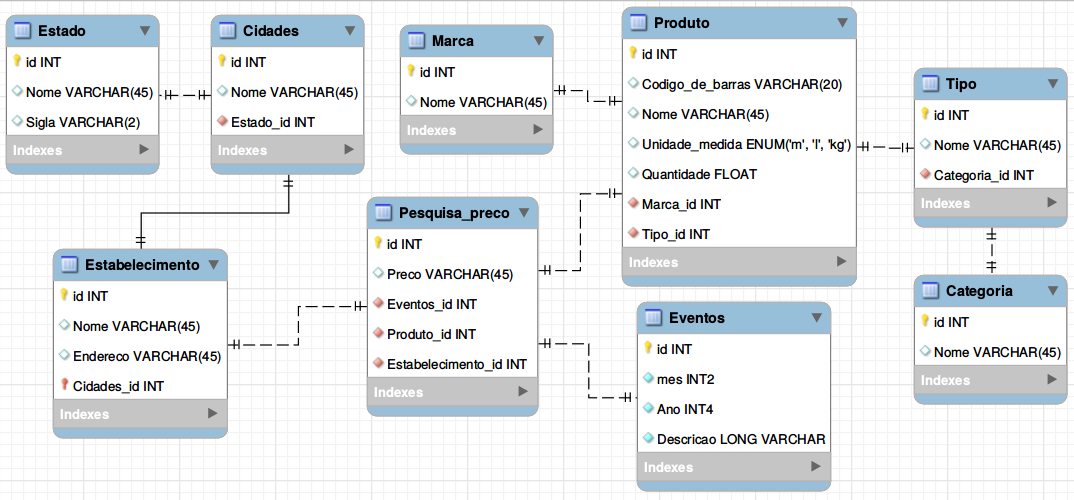
\includegraphics[width=16.0cm, height= 9.0cm]{cestadiagrama.png}    % The printed column width is 8.4 cm.
		Fonte: Autor
		\caption{Diagrama de Entidade e Relacionamento.} 
		
		\label{fig:faces}
	\end{center}
\end{figure}
As informações foram colocadas de forma a relacionar o máximo possível, mesmo o sistema atendendo atualmente somente a cidade de paraíso foi colocado cidade e estado para que se o sistema for expandir para outras localidades o banco já está configurado.

Os produtos foram separados das marcas para facilitar na mineração de dados futuramente, para que se tenha uma noção de preferência sobre os gostos dos consumidores, pois um dos objetivos futuros quando o sistema já tiver uma boa quantidade de dados é fazer mineração de dados.



	
\chapter{Desenvolvimento}
	
O desenvolvimento do projeto deu se inicio com a verificação de todos os dados já coletados da cesta básica, onde se encontravam em uma planilha eletrônica, em seguida foi feito o planejamento do sistema em cima da metodologia utilizada para a coleta dos dados, depois de compreender como os dados deveriam ser estruturados e a aplicação deveria funcionar e que começou o desenvolvimento com o \textit{framework} Django.

O Django possui uma estrutura bem simples de utilização, criando o arquivo de Model e descrevendo toda a modelagem do banco de dados na sua tela administrador onde é possível fazer toda a gerência dos dados, sem precisar programar toda a estrutura do CRUD.

\begin{figure}[H]
	\begin{center}
		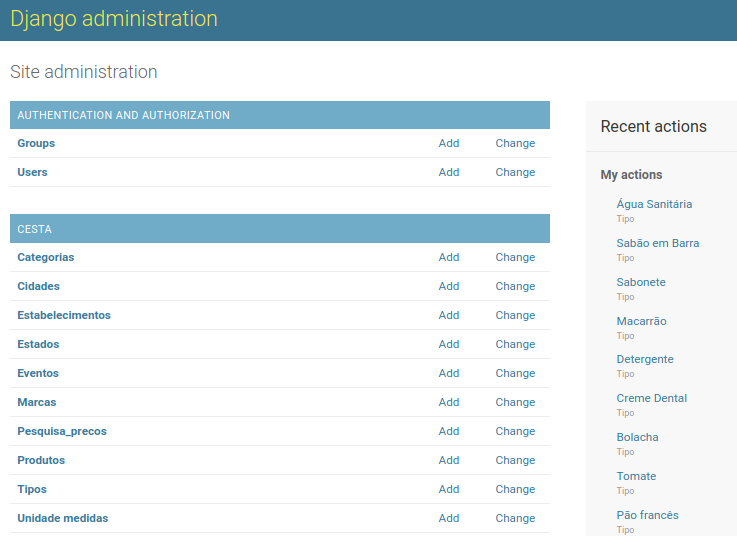
\includegraphics[width=16.0cm, height= 7.0cm]{cestaadmin.png}    % The printed column width is 8.4 cm.
		Fonte: Autor
		\caption{Tela administrador do Django.} 
		\label{fig:faces}
	\end{center}
\end{figure}
Com isso foi aproveitado a parte de gerência de dados e usuários, não sendo necessário programar essa parte, no entanto para quem vai pesquisar os preços utilizando essa estrutura não ficaria fácil, pois seria necessário ter que fazer vários relacionamentos de dados manualmente.

Para quem faz a pesquisa de preço foi programado um módulo que facilite, de forma que inicialmente ele pudesse escolher a data, o estabelecimento, o tipo do produto, com isso ele só irá precisar escolher o produto e colocar o preço.

\begin{figure}[H]
	\begin{center}
		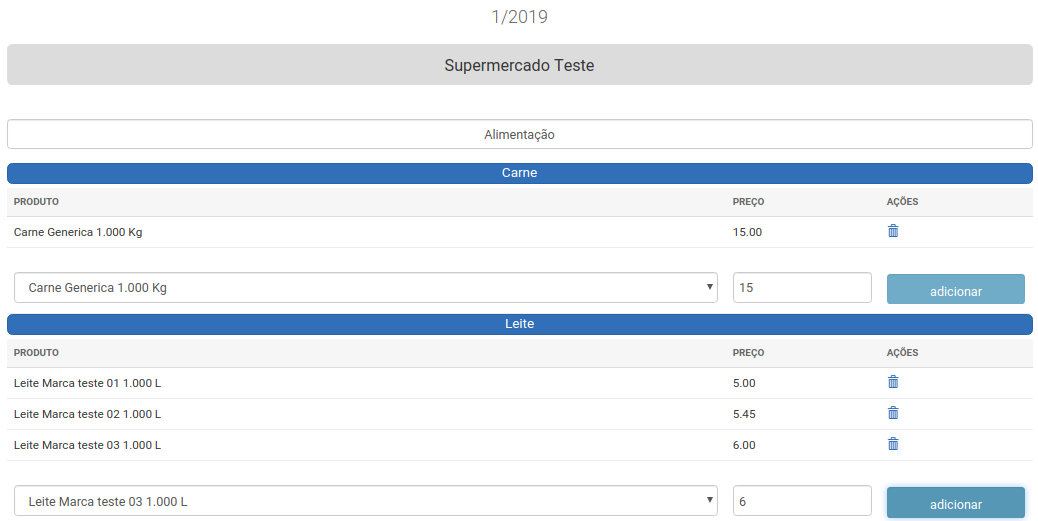
\includegraphics[width=16.0cm, height= 8.0cm]{cestacadastro.png}    % The printed column width is 8.4 cm.
		Fonte: Autor
		\caption{Tela de Registro de Preços Pesquisados} 
		\label{fig:faces}
	\end{center}
\end{figure}

Para o Layout do visitante foi planejado um template amigável e responsivo de forma que pudesse se adaptar a qualquer resolução de tela.


\begin{figure}[!h]
	\begin{center}
		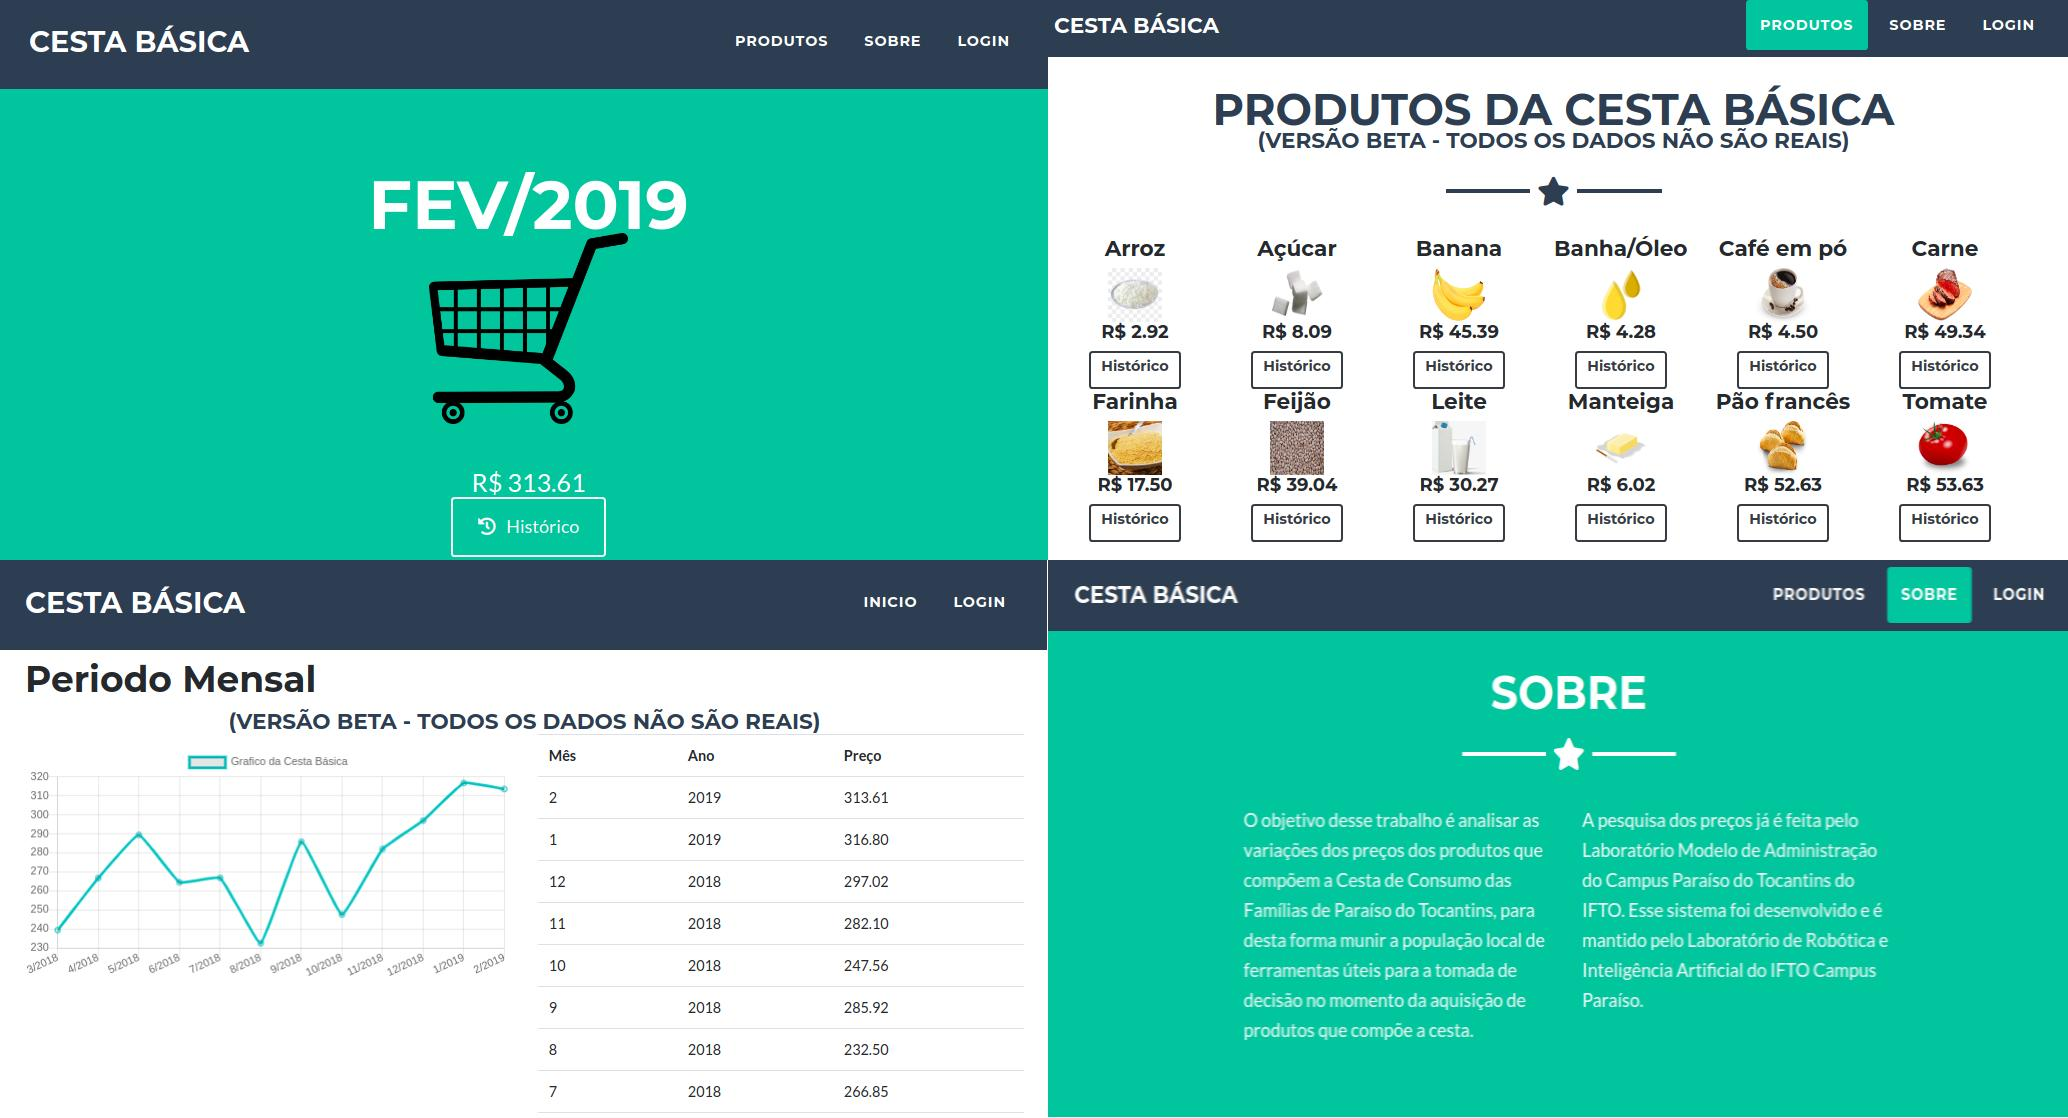
\includegraphics[width=16.0cm, height= 8.0cm]{cestauser.jpeg}    % The printed column width is 8.4 cm.
		Fonte: Autor
		\caption{Tela para visualização dos dados para os usuários} 
		\label{fig:faces}
	\end{center}
\end{figure}

O sistema \textit{Web} foi hospedado dendo dos servidores do IFTO, no projeto foi escolhido o SQLite para ser o banco de dados, no entanto, a hospedagem oferecida no servidor foi o MySql, algumas modificações tiveram que serem feitam para adaptar-se ao banco, mais por ambos serem bancos de dados relacionais não houve impacto no projeto e foi hospedado com sucesso.

Após a conclusão do sistema \textit{Web} foi dado início ao planejamento do aplicativo, a proposta do aplicativo é que ele possa ser usado mesmo sem internet, então foi feito o desenvolvimento de uma API no sistema \textit{Web} para que o aplicativo possa baixa os dados e salvar localmente no dispositivo do usuário.

Para fazer o desenvolvimento do aplicativo foi escolhido o \textit{framework} Flutter, pois ele permitir desenvolver em linguagem nativa tanto para Android e iOS. Devido aos alto custo para colocar o aplicativo na \textit{Apple Store} foi decidido não lançar o aplicativo para essa plataforma, apenas foi lançado o aplicativo para Android na \textit{Play Store}.

\begin{figure}[!h]
	\begin{center}
		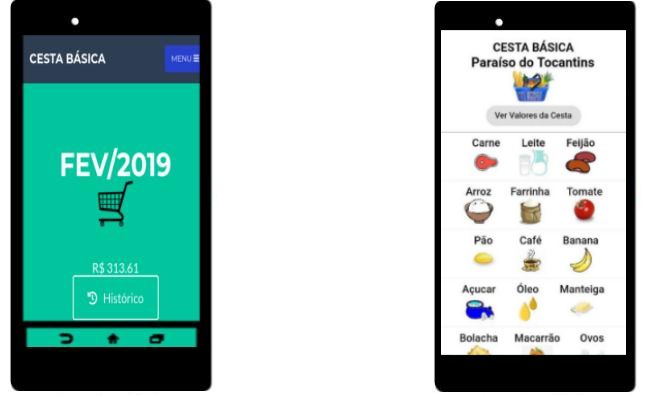
\includegraphics[width=12.0cm, height= 8.0cm]{movel.png}    % The printed column width is 8.4 cm.
		
		Fonte: Autor
		\caption{Demonstração do sistema \textit{Web} rodando em dispositivo móvel e a interface principal do aplicativo.} 
		\label{fig:faces}
	\end{center}
\end{figure}

O aplicativo foi desenvolvido utilizando um \textit{layout} diferente do sistema \textit{Web}, o aplicativo foi planejado para ser mais simples, e foram deixados fora varias funções que não são necessárias para os usuários, o aplicativo apenas permite ver o histórico da Cesta Básica e dos produtos em forma de tabela.

O aplicativo pega os dados do servidor \textit{Web} através de uma API, após a primeira conexão do aplicativo ao servidor \textit{Web} os dados ficam armazenados no aplicativo, com os dados no aplicativo é possível acessá-los mesmo sem internet.

\chapter{Considerações finais}
No início desse projeto houve várias discussões sobre os meios que seriam utilizados para se alcançar o
resultado, o resultado que era esperado foi definido no início do projeto, no entanto, os meios para atingir os
resultados foram planejados depois que começou o projeto através de várias discussões sobre quais deveriam ser as
melhores práticas e ferramentas para o desenvolvimento.

Houve a necessidade por parte do desenvolvedor de aprender a utilização dos \textit{frameworks} Django e Flutter que ainda
não era do seu conhecimento, mas isso não foi um grande empecilho para o projeto, pois o tempo de duração do
projeto era suficiente para aprendizado das ferramentas e o desenvolvimento, as outras ferramentas utilizadas já eram
de conhecimento do desenvolvedor e apenas alguns detalhes a mais tiveram que ser buscado para o
desenvolvimento.

Não foi um objetivo deste trabalho analisar os dados coletados da cesta básica, esse trabalho foi focado
apenas no desenvolvimento das plataformas, a análise dos dados será proposta para os alunos, a inserção e atualização de novos dados ficará de responsabilidade dos alunos do
curso de administração. Devido a falta de voluntários para a coleta dos dados, houve uma pausa no projeto em julho de 2019 e até dessa publicação ainda não houve retorno na coleta dos dados.

Pode-se dizer que o sistema e o aplicativo proposto nesse trabalho foi alcançado, apesar de que ainda podem ser
melhorados, o objetivo principal que embasa o sistema foi concluído, novas funções podem ser adicionadas para
torná-lo ainda mais eficiente.

O sistema apesar de em seu escopo foi definido para apenas Paraíso do Tocantins, sua base do banco de
dados permite uma expansão para outras cidades, a proposta futura desse projeto é uma expansão de sua atuação
para mais localidades.

% Finaliza o bookmarking do PDF
\phantompart

% ------------------------------------------------------------------------------
% ELEMENTOS PÓS-TEXTUAIS
% ------------------------------------------------------------------------------

% Introduz a parte pós-textual
\postextual

% Insere as referências bibliográficas
\bibliography{bibliografia}

% ----------------- APÊNDICES -----------------
%\begin{apendicesenv}
	
%	\partapendices
	
%	\chapter{Título do Apêndice}
	
%		Documento ou texto “elaborado” pelo autor, inserido ou referido no trabalho a fim de complementar a sua argumentação. Para	não haver prejuízo à unidade nuclear do	trabalho, cópia integral do documento é	acrescida ao final.
		
%	\chapter{Outro Apêndice}
	
%		Outro documento ou texto “elaborado” pelo autor, inserido ou referido no trabalho a fim de complementar a sua argumentação. Para	não haver prejuízo à unidade nuclear do	trabalho, cópia integral do documento é	acrescida ao final.
	
	% Inserir outros apêndices caso seja necessário ...
	
%\end{apendicesenv}


% ----------------- ANEXOS -----------------
%\begin{anexosenv}
	
%	\partanexos
	
%	\chapter{Título do Anexo}
	
%		Documento ou texto “não elaborado”	pelo autor, inserido ou referido no trabalho, a fim de fundamentar, comprovar ou ilustrar a sua argumentação. Igualmente, para não haver prejuízo à unidade nuclear do trabalho, cópia integral do documento é acrescida ao final do trabalho.
		
%	\chapter{Outro Anexo}
	
		%Outro documento ou texto “não elaborado”	pelo autor, inserido ou referido no trabalho, a fim de fundamentar, comprovar ou ilustrar a sua argumentação. Igualmente, para não haver prejuízo à unidade nuclear do trabalho, cópia integral do documento é acrescida ao final do trabalho.
	
%\end{anexosenv}

\end{document}
